\documentclass[../main.tex]{subfiles}

\newcommand{\rot}{\text{rot}}

\begin{document}
    \chapter{Плазмонные эффекты в HgCdTe}
    
    Плазмоны - это квазичастицы, отвечающие квантованию 
    Ленгмюровских колебаний. Они в значительной мере 
    определяют оптические свойства материалов, в том числе 
    гетероструктур на основе $Hg_xCd_{1-x}Te$.

    \section{Электродинамические свойства двумерных плазмонов}

    Плазмоны представляют собой TM волны, имеющие одну компоненту 
    магнитного поля и две компоненты электрического. Они распространяются 
    вдоль проводящего слоя. Схематичное изображение поля приведено на 
    Рис. \ref{plasmons:schematic:fiels} 

    \begin{figure}[h]
        \begin{minipage}[h]{1\textwidth}
            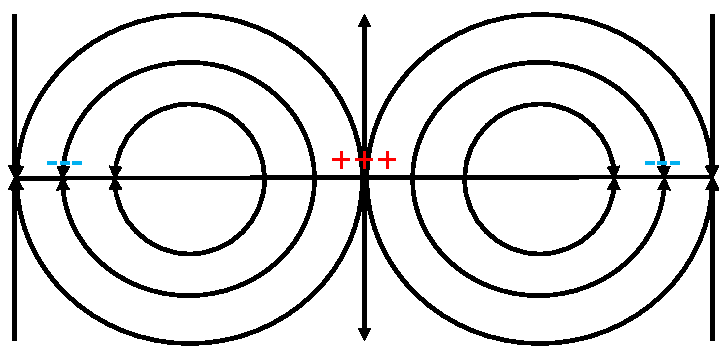
\includegraphics[width=0.7\textwidth]{./images/schematic_field.pdf}
            \caption{Схематичное изображения распределения поля плазмона.
            \label{plasmons:schematic:fiels}}
        \end{minipage}
    \end{figure}

    Рассмотрим свойства плазмонов, в предположении, что ток,
    соответствующий им локализован в квантовой яме и течет только
    в плоскости. Аппроксимация $\delta$ функцией является 
    справедливой, поскольку характерная длина волны имеет порядок 
    единиц $\mu\text{m}$, a толщина квантовой ямы - порядок единиц 
    $\text{nm}$. Тогда из уравнений Максвелла:
    \begin{equation}
        \rot \vec H = \frac{\varepsilon}{c} \dot{\vec E} + \delta(z) \vec j;
    \end{equation}

    Предположим, что ток обусловлен исключительно электрическим полем
    $\vec j  = \sigma \vec E$ и сделаем предположения о направлениях 
    $\vec j \parallel \vec E \parallel \vec{x}_0, \vec H \parallel \vec{y}_0$.
    Распишем покомпонентно:
    \begin{equation}
        \begin{aligned}
            \partial_x H_y &=& \frac{\varepsilon}{c} \dot{E}_z;
            -\partial_z H_y &=& \frac{\varepsilon}{c} \dot{E}_x + \frac{4\pi };
        \end{aligned}
    \end{equation}

    Принимая во внимание уравнение на электрическое поле:
    \begin{equation}
        \rot \vec E = \frac{1}{c} \dot \vec H;
    \end{equation}

    Сделаем его Фурье преобразование в плоскости квантовой ямы
    и получим замкнутую систему уравнений:
    \begin{equation}
        \left\{
        \begin{aligned}
            - i \frac{\omega}{c} H_y &=& i k E_z - \partial_z E_x;\\
            - \partial_z H_y  &=& \frac{4\pi}{c} \underbrace{\sigma E_x}_{\vec j} 
            - i \varepsilon  \frac{\omega}{c} E_x;\\
            ik H_y  &=& - i \varepsilon \frac{\omega}{c} E_z;
        \end{aligned}
        \right.
    \end{equation}

    Решая её получим уравнение на зависимость поля от $z$:
    \begin{equation}
        \frac{\partial^2 E_x}{\partial z^2} = \frac{4\pi i}{\varepsilon \omega}
        \underbrace{\left(k^2  - \varepsilon \frac{\omega^2}{c^2}\right)}_{q^2} \sigma E_x \delta(z)
        + \underbrace{\left(k^2  - \varepsilon \frac{\omega^2}{c^2}\right)}_{q^2} E_x;
    \end{equation}

    Предположим решение в виде спадающих от квантовой ямы экспонент
    с волновым вектором $i\alpha$:
    \begin{equation*}
        E_x = \left\{
            \begin{aligned}
                E_0 \exp{-\alpha z} & &z > 0\\
                E_0 \exp{\alpha z} & &z < 0
            \end{aligned}
        \right.;
    \end{equation*}

    Интегрируя в окрестности нуля получим граничное условие на на производные:
    \begin{equation*}
        \left.\frac{\partial E_x}{\partial z}\right\vert{}^{+0}_{-0} = \frac{4\pi i}{\varepsilon \omega}
        \left(k^2  - \varepsilon \frac{\omega^2}{c^2}\right);
    \end{equation*}

    Отсюда можно получить дисперсионное соотношение для таких двумерных плазмонов:
    \begin{equation}
        \label{plasmons:disp}
        k^2  = \varepsilon  \frac{\omega^2}{c^2} - \left(\frac{\varepsilon\omega}{2\pi \sigma}\right)^2;
    \end{equation}
    
    \section{Дисперсионные соотношения плазмонов}

    Поскольку речь идёт о квантовании классических ЭМ колебаний, 
    для получения дисперсионного соотношения необходимо найти 
    материальные соотношения, а в частности - зависимость 
    диэлектрической проницаемости от частоты и волнового вектора.

    Выражение для поправки к диэлектрической проницаемости является 
    обобщением т.н. формулы Линдхарда (учитывается несколько зон, в то 
    время как сам Линдхард работал в однозонном приближении)
    и приведено ниже:
    \begin{equation}
        \label{lindhard}
        \kappa_{pl}(\vec q, \omega) = \frac{4\pi}{\vec{q}^2 V}
            \sum_{m, n} \int d\vec k \frac{f_m(\vec k) - f_n(\vec k 
                + \vec q)}{\varepsilon_n(\vec k + \vec q) - 
                \varepsilon_m - \hbar \omega - \i \hbar \alpha}
                \bra{\psi_{\vec k + \vec q,n}} \ket{\psi_{\vec k, m}};
    \end{equation}

    Ленгмюровские колебания являются колебаниями поляризации. Таким
    образом они должны подчиняться уравнению связи поляризации и 
    плотности свободного заряда $\div \vec P  = - \rho$. Кроме того 
    такие колебания могут возбуждаться внешним электрическим полем, 
    которое мы примем потенциальным $\vec E = - \grad \varphi$ и 
    гармоническим. Тогда оно будет давать добавку потенциальной энергии:
    \begin{equation}
        \label{plazmon:field}
        \hat \varphi  = U \exp{i\vec q \vec r - i \omega t}
            + U^{\dagger} \exp{-i\vec q\vec r + i \omega t};
    \end{equation}

    В общем виде функции представляются в виде огибающей, зависящей 
    от времени и быстроосциллирующего члена. В частности:
    \begin{equation}
        \label{plasmons:wf0}
        \ket{\vec k, m} = \frac{1}{\sqrt S} \exp{i\vec k \vec r}
            \exp{-i \omega_{\vec k, m} t} \psi_{\vec k, m};
    \end{equation}

    Здесь $\vec k$ - волновой вектор, которому отвечает функция, 
    $m$ - номер подзоны с учётом спина и размерного квантования 
    по оси $z$. $\psi_{\vec k, m}$ - волновые функции
    \ref{calculation:wf}, полученные по методике, 
    описанной в прошлой главе \ref{chapter:calcs}. 

    Электрическое поле в виде \ref{plazmon:field} должно вызывать 
    искажения 
    такой равновесной волновой функции с волновыми векторами
    $\vec k \pm \vec q$, т.e. в первом порядке малости по полю:
    \begin{equation}
        \label{plasmons:wf1}
        \psi_m (\vec k, \vec r) = \ket{\vec k, m} + \sum_n b_{\vec k 
            + \vec q, m, n} (t) \ket{\vec k + \vec q, n} + \sum_n 
            c_{\vec k - \vec q, m, n} (t) \ket{\vec k - \vec q, n};
    \end{equation}

    В таком случае плотность заряда может быть записана как:
    \begin{multline}
        \label{charge_density}
        \rho = -e \sum_{m} \int d\vec k  \left(
            \bra{\psi_m (\vec k, \vec r}\ket{\psi_m (\vec k, 
            \vec r} - 1\right) f_m(\vec k) =
            \sum_{m, n} \int d \vec k f_m (\vec k) \\
            \left( b_{\vec k + \vec q, m, n} (t)
            \bra{\vec k, m} \ket{\vec k 
            + \vec q, n} + b^\dagger_{\vec k + \vec q, m, n} (t) 
            \bra{\vec k + \vec q, n} \ket{\vec k, m}\right.\\ 
            \left. + c_{\vec k - \vec q, m, n} (t) \bra{\vec k, m} 
            \ket{\vec k  - \vec q, n} + c^\dagger_{\vec k - \vec q, m, n} 
            (t) \bra{\vec k - \vec q, n} \ket{\vec k, m} \right);
    \end{multline}
    
    Для получения коэффициентов $b,~c$ воспользуемся нестационарной 
    теорией возмущений.

    Результатом для вычисления коэффициентов является:
    \begin{equation}
        \label{plasmons:charge:coeffs}
        \begin{aligned}
            b_{\vec k + \vec q, m, n} (t) = U \frac{\exp{-i\omega t - i 
                \varepsilon_m (\vec k) t / \hbar + i \varepsilon_n(\vec k 
                + \vec q) t / \hbar + \alpha t}}{\varepsilon_m (\vec k) + \hbar 
                \omega - \varepsilon_n(\vec k + \vec q)+ i \hbar \alpha}
                \bra{\psi_{\vec k+\vec q, n}}\ket{\psi_{\vec k, m}}; \\
            c_{\vec k - \vec q, m, n} (t) = U^\dagger \frac{\exp{i\omega t - i 
                \varepsilon_m (\vec k) t / \hbar + i \varepsilon_n(\vec k 
                - \vec q) t / \hbar + \alpha t}}{\varepsilon_m (\vec k) - \hbar 
                \omega - \varepsilon_n(\vec k - \vec q)+ i \hbar \alpha}
                \bra{\psi_{\vec k+\vec q, n}}\ket{\psi_{\vec k, m}};
        \end{aligned}
    \end{equation}

    В частности, стоит отметить, что для случая квантовой ямы, скалярное 
    произведение функций вида $\psi_{k, m}$ будет содержать в том числе 
    и скалярное произведение по оси $z$. Предполагая квантованность по 
    этой оси:
    \begin{multline}
        \bra{\psi_{\vec q, n}}\ket{\psi_{\vec k, m}} = 
            \bra{\sum_i \exp{k_{z,i} \sum_j c_{nij \vec q}} u_j(\vec r)}
            \ket{\sum_i \exp{k_{z,i} \sum_j c_{mij \vec k}} u_j(\vec r)}\\ 
            = \sum_{s=\{i,j\}}  c^\dagger_{ns \vec q} c_{ms \vec k};
    \end{multline}

    Подставляя полученные выражения в \ref{charge_density} 
    и приводя подобные можно получить:
    \begin{multline}
        \rho = \frac{e^2 U}{S} \exp{i\vec q \vec r - i \omega t + \alpha t}
            \sum_{m, n} \int d\vec k \left( \frac{\bra{\psi_{\vec k + \vec q, n}}
            \ket{\psi_{\vec k, m}}}{\varepsilon_m(\vec k) + \hbar \omega - 
            \varepsilon_n(\vec k + \vec q) + i \hbar \alpha} +\right. \\ 
            \left. \frac{\bra{\psi_{\vec k - \vec q, n}}
            \ket{\psi_{\vec k, m}}}{\varepsilon_m(\vec k) - \hbar \omega - 
            \varepsilon_n(\vec k - \vec q) - i \hbar \alpha} \right) + \text{c.c.}=\\
            \frac{e^2 U}{S} \exp{i\vec q \vec r - i \omega t + \alpha t}
            \sum_{m, n} \int d\vec k \bra{\psi_{\vec k + \vec q, n}}
            \ket{\psi_{\vec k, m}} \frac{f_m(\vec k) - f_n(\vec k - \vec q)}
            {\varepsilon_m(\vec k) + \hbar \omega - \varepsilon_n(\vec k + \vec q) 
            + i \hbar \alpha};
    \end{multline}

    Учитывая это выражение мы получаем формулу Линдхарда \ref{lindhard}. Обладая 
    этим знанием сравнительно легко получить дисперсионное соотношение для плазмонов
    \ref{plasmons:disp}, решая следующее уравнение:
    \begin{equation}
        \label{plasmons:disp}
        \frac{1}{(2\pi)^2}\frac{\kappa^2}{\kappa^2_{pl}} = 
        \vec{q}^2 - \kappa \frac{\omega^2}{c^2};
    \end{equation}
    
    Очевидно, что это уравнение может иметь мнимые корни. Причём, как правило,
    численно удобнее решать это уравнение, задавая частоту и решая относительно 
    волнового вектора.

    За счёт фононного вклада \cite{palik1998handbook} \ref{plasmons:phonons} в 
    диэлектрическую проницаемость это уравнение обладает двумя решениями, 
    отвечающими "нижней" и "верхней" ветвям дисперсионного соотношения.

    \begin{equation}
        \label{plasmons:phonons}
        \kappa_{ph}(\omega) = \left(
            1 + \frac{\omega_L^2 - \omega_T^2}{\omega_T^2-\omega^2 + i \Gamma \omega}
            \right);
    \end{equation}

    Оказывается LO фононы и плазмоны могут взаимодействовать за счет продольной компоненты поля.
    В объемном материале эта задача была рассмотрена в \cite{peter2002manuel}. 

    \section{Результаты расчёта спектра плазмонов}

    В дальнейшем будут показаны зонные спектры плазмонов "верхней" ветки в 
    квантовой яме толщиной $6~\text{nm}$, имеющую состав ямы $HgTe$ и 
    барьеров $CdTe$. При этом структура полагается выращенной в кристаллографическом
    направлении [013], а температура решётки и температура носителей заряда равной 
    температуре жидкого гелия $4.2~\text{K}$. Продемонстрированны срезы 
    $\vec k = (k_x, 0)$.

    \begin{figure}[h]
        \begin{minipage}[h]{0.49\textwidth}
            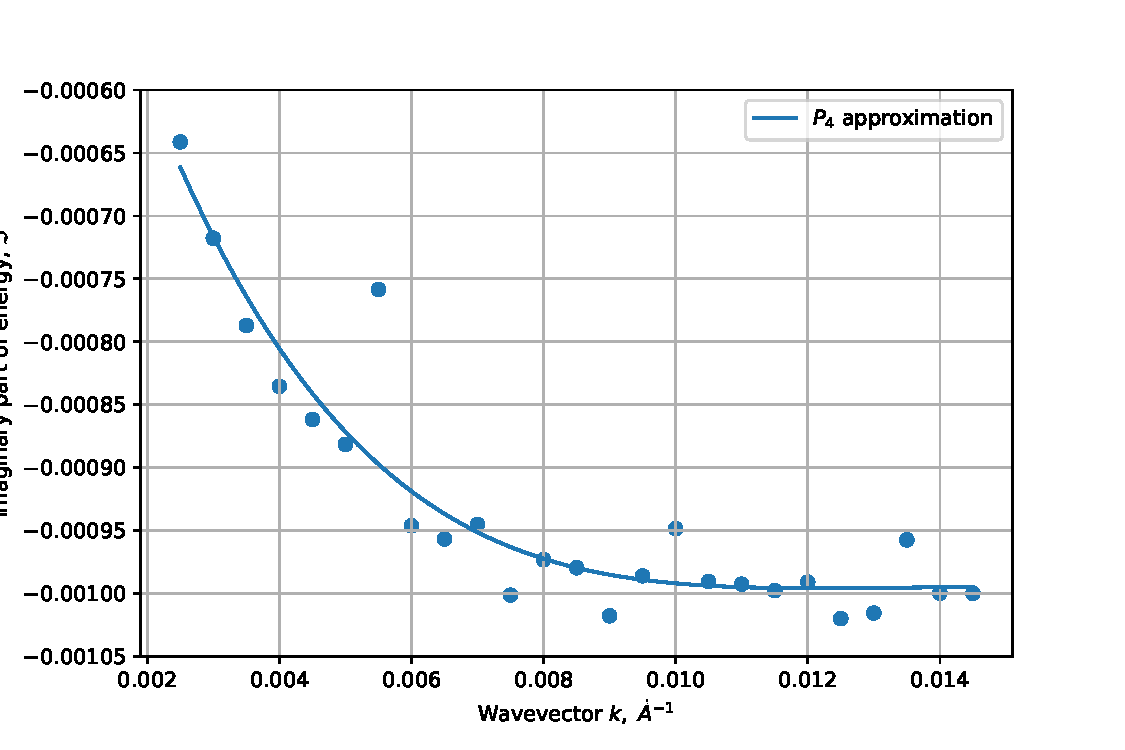
\includegraphics[width=0.9\textwidth]{./images/plasmon_6nm_25_001_im.pdf}
            \caption{Мнимая часть частоты в зависимости от волнового вектора, при $N_e = 2.5 \cdot 10^{11}~\text{cm}^{-2},~N_h = 10^9~\text{cm}^{-2}$
            \label{plasmon:6nm25ne001npim}}
        \end{minipage}
        \hfill
        \begin{minipage}[h]{0.49\textwidth}
            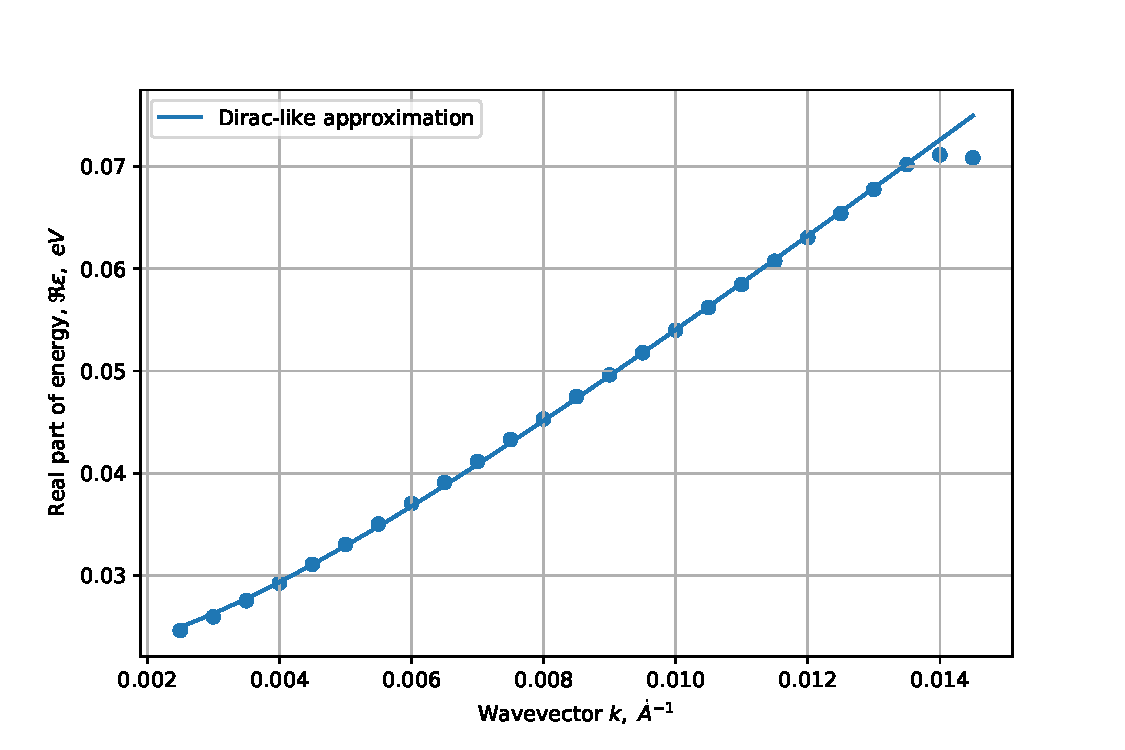
\includegraphics[width=0.9\textwidth]{./images/plasmon_6nm_25_001_re.pdf}
            \caption{Действительная часть частоты в зависимости от волнового вектора, при $N_e = 2.5 \cdot 10^{11}~\text{cm}^{-2},~N_h = 10^9~\text{cm}^{-2}$
            \label{plasmon:6nm25ne001npre}}
        \end{minipage}
    \end{figure}

    На представленных выше графиках \ref{plasmon:6nm25ne001npim}, \ref{plasmon:6nm25ne001npre} видно видно несколько особенностей.
    В частности заметно, что в данном случае плазмоны могут лишь затухать, поскольку нет достаточной инверсии населенности. 
    Также видно, что мнимая часть частоты вычисляется неустойчиво (т.е. "выбросы" на Рис. \ref{plasmon:6nm25ne001npim} 
    являются артефактами численного расчёта).

    Однако при некоторых условиях плазмоны могут иметь и положительную мнимую часть частоты, что соответствует усилению плазмонов. Для того, 
    чтобы эти условия удовлетворялись необходимо, чтобы в полупроводнике была существенная инверсия населенности, а энергия плазмона была больше 
    эффективной ширины запрещенной зоны \cite{kapralov2019feasibility}. 

    При низкой концентрации энергия плазмонов будет меньше эффективной ширины запрещённой зоны. С увеличением концентрации
    равновесных носителей заряда растет и энергия плазмоны при заданном волновом векторе $\vec q$. Таким образом повышая концентрацию
    равновесных носителей можно снизить пороговую концентрацию неравновесных. 
    
    Такие явления могут наблюдаться, к примимеру, после накачки. 
    Особый интерес представляет "граница" концентрации, при которой будет наблюдатьтся усиление. Одно из таких дисперсионных соотношений 
    приведено ниже на Рис. \ref{plasmon:6nm3ne0125npim}, \ref{plasmon:6nm3ne0125npre}.

    \begin{figure}[h]
        \begin{minipage}[h]{0.49\textwidth}
            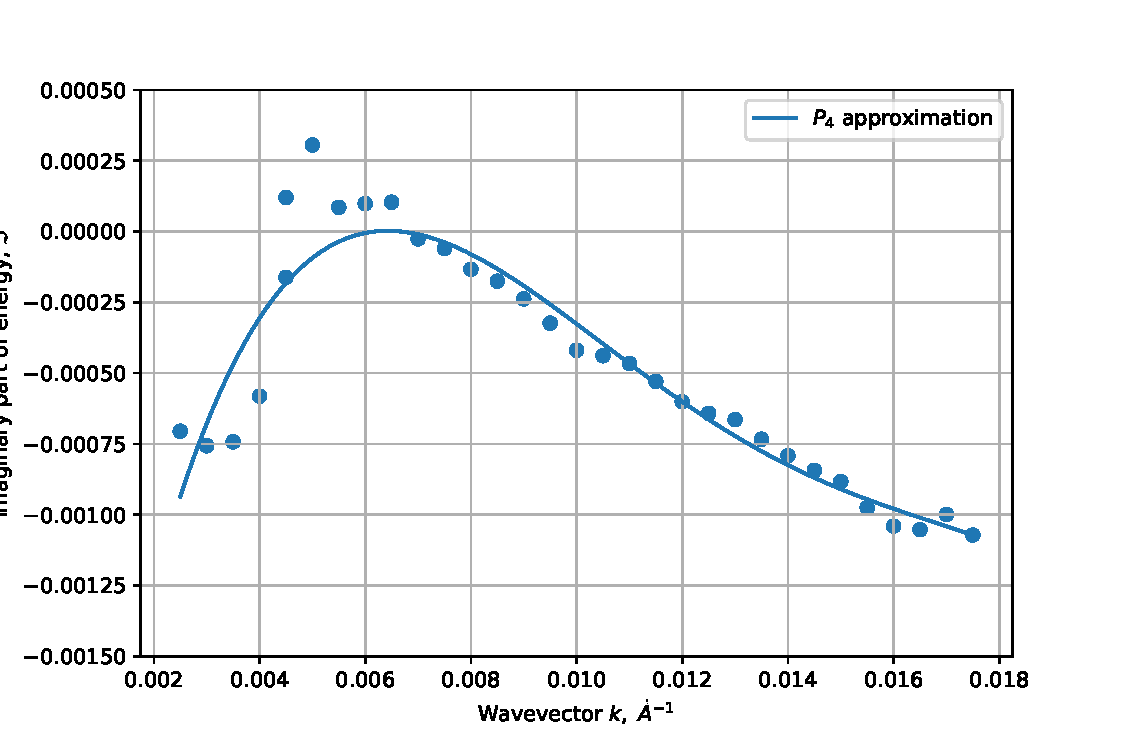
\includegraphics[width=0.9\textwidth]{./images/plasmon_6nm_3_0125_im.pdf}
            \caption{Мнимая часть частоты в зависимости от волнового вектора, при $N_e = 3 \cdot 10^{11}~\text{cm}^{-2},~N_h = 1.25 \cdot 10^{10}~\text{cm}^{-2}$
            \label{plasmon:6nm3ne0125npim}}
        \end{minipage}
        \hfill
        \begin{minipage}[h]{0.49\textwidth}
            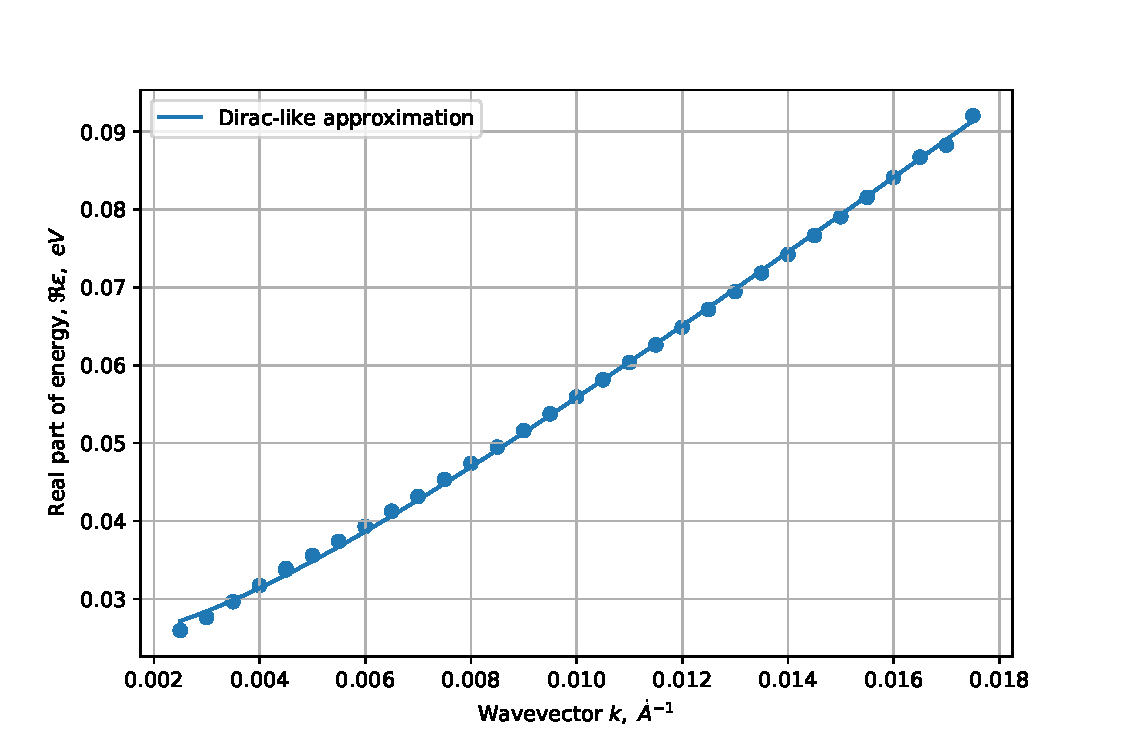
\includegraphics[width=0.9\textwidth]{./images/plasmon_6nm_3_0125_re.pdf}
            \caption{Действительная часть частоты в зависимости от волнового вектора, при $N_e = 3 \cdot 10^{11}~\text{cm}^{-2},~N_h = 1.25 \cdot 10^{10}~\text{cm}^{-2}$
            \label{plasmon:6nm3ne0125npre}}
        \end{minipage}
    \end{figure}

    Для того чтобы оценить, что действительно существует порог можно посмотреть на сводную диаграмму для семейства зависимостей $\Im \omega(\vec q)$
    (мнимой части дисперсионных соотношений) при постоянной концентрации электронов и изменяющейся концентрации дырок \ref{plasmon:6nm3neXnpim}.
    Стоит отметить, что именно эта зависимость определяет коэффициент усиления/поглощения:
    \begin{equation}
        \alpha(\Re \omega (\vec q)) = -2 \Im \omega \Re \left(\frac{d\omega}{d\vec q}\right)^{-1};
    \end{equation}

    \begin{figure}[h]
        \begin{minipage}[h]{1\textwidth}
            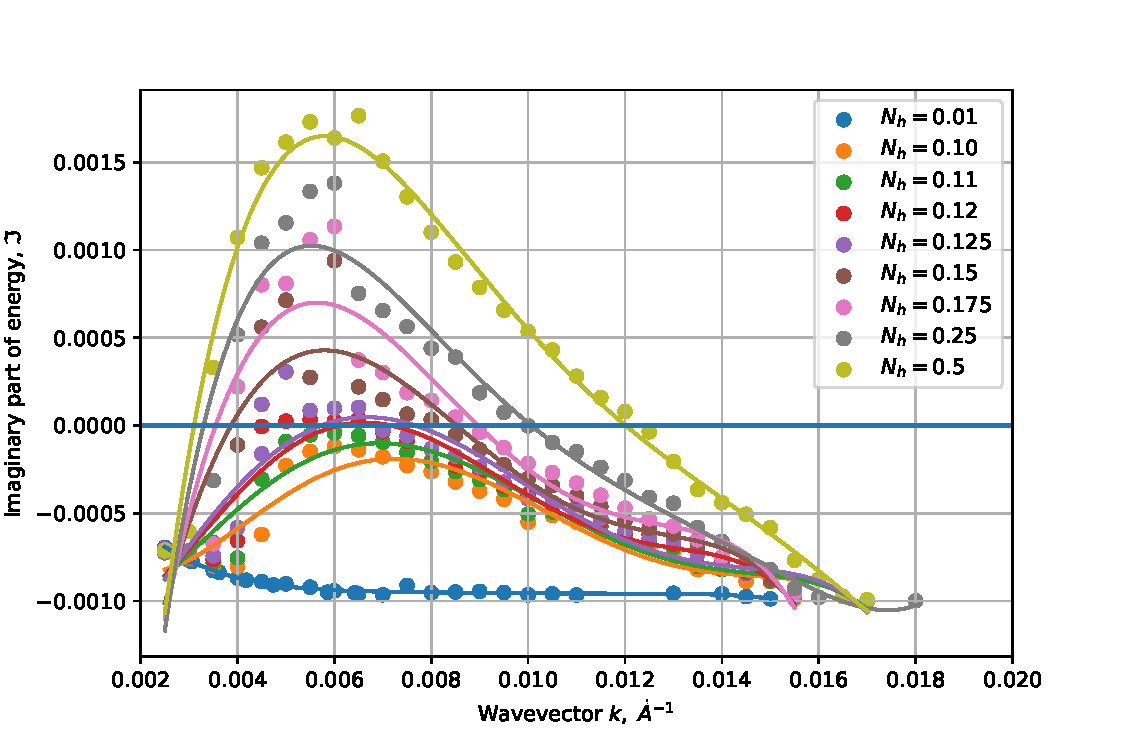
\includegraphics[width=1\textwidth]{./images/plazmon6nm3neXnpim.pdf}
            \caption{Мнимая часть частоты в зависимости от волнового вектора, при $N_e = 3 \cdot 10^{11}~\text{cm}^{-2},~N_h = x \cdot 10^{10}~\text{cm}^{-2}$,
            где $x$ указан на графике.\label{plasmon:6nm3neXnpim}}
        \end{minipage}
    \end{figure}
    

\end{document}